\clearpage
\section{実験内容 (2)}

様々なサーバソフトウェアを動作させるためには,オペレーティングシステムに対して適切なネットワーク設定を行う必要がある.サーバは通常アプリケーション層(あるいはセッション層以上)で動作するため,必要なネットワーク設定は,物理層からネットワーク層(実質はトランスポート層)までの設定である.

そこで,インストールされたOSに対して,イーサネットとIPネットワークの設定を行う.
\begin{enumerate}
 \item もしコンピュータにネットワークインターフェースが認識されていない
       場合は,ネットワークインターフェースのハードウェアの種類と,使用
       するOSのバージョンに合致したデバイスドライバをインストールする.
 \item ネットワークケーブルを用意し,レイヤー2スイッチに適切に接続する.UTP カテゴリ5の場合は,
       適切な長さのケーブルを作成することができる.
 \item ネットワークインターフェースに IP アドレス・サブネットマスク・デフォ
       ルトゲートウェイ,DNSサーバを設定する.
 \item インターネットへ接続ができるようにする
 \item 下記ネットワーク管理に有用なソフトウェアをインストールする
 \begin{itemize}
     \item Linux: net-tools, telnet, traceroute
     \item Windows: Putty, WinSCP
     \item ChromeOS: Linux (ping, ssh等) を使えるようにする.Android アプリが使えるようにする.「Wifi Analyzer」をインストール
 \end{itemize}
 \item 全ての端末から,全てのユーザ名で,ssh でログインできるようにする.
\end{enumerate}

まず,図\ref{fig:01:system}を参照し,各グループに必要なLANケーブルを準備
する.作成したLANケーブルで各機器を正しく接続した後,IPアドレス,サブネッ
トマスク,デフォルトゲートウェイ,DNSサーバなどの設定を行い,各機器が通
信を行える環境を構築する.また,外部Webサイトを閲覧できるように,各クラ
イアントPCのブラウザにHTTP Proxyサーバの設定を行う.

\begin{figure}[tb]
    \centering
        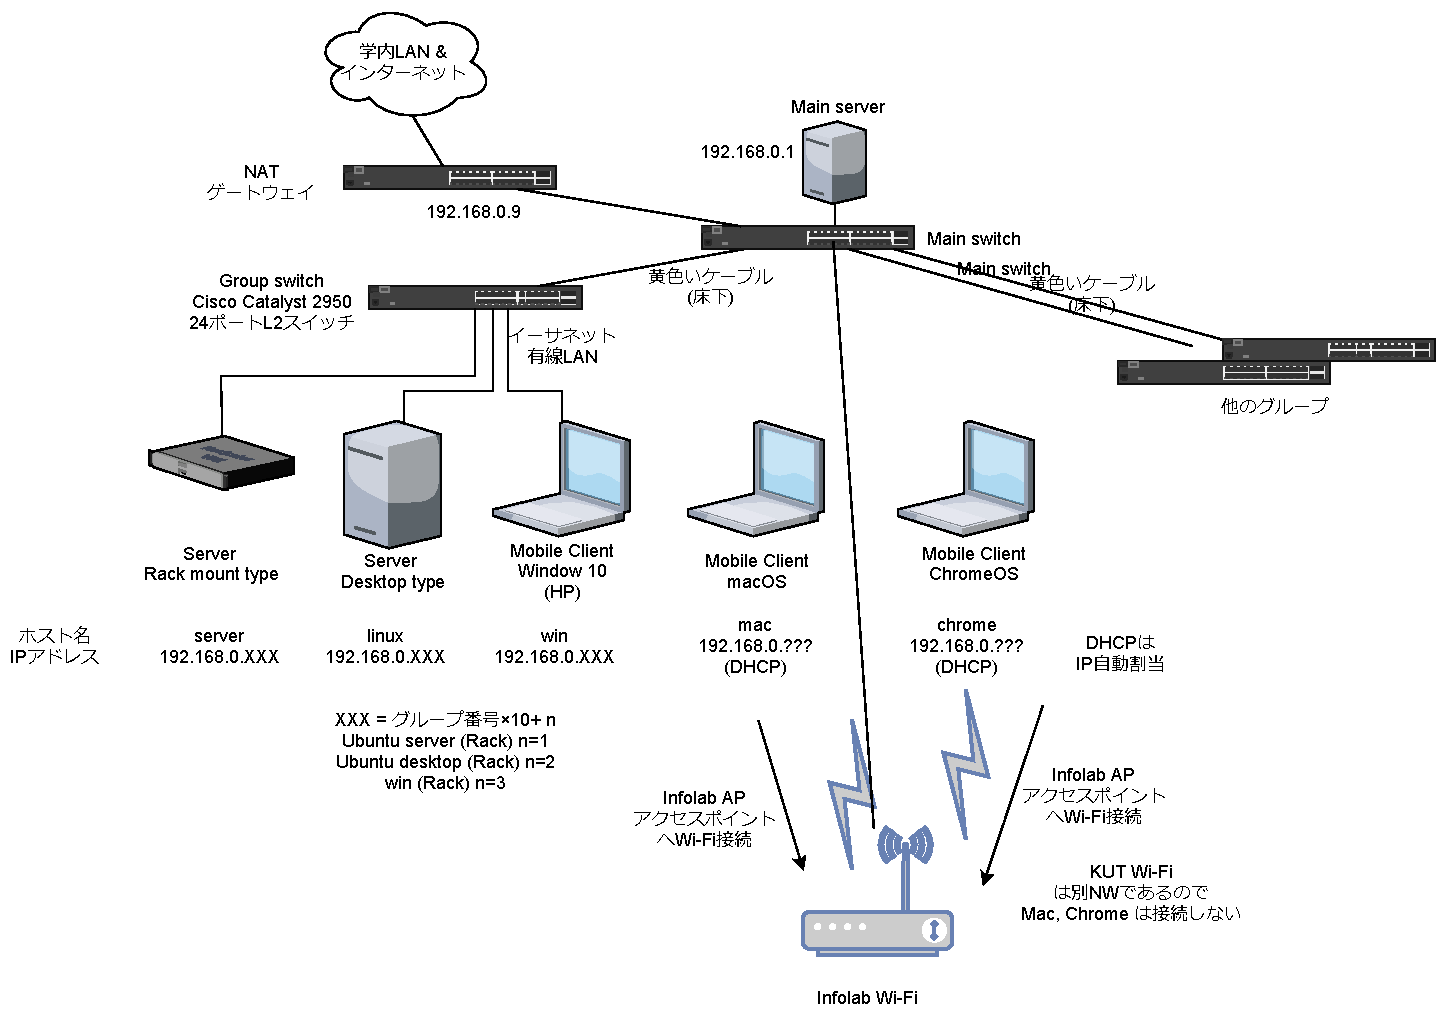
\includegraphics[width=\textwidth]{01_os/system-network.pdf}
        \caption{各グループのネットワーク接続図とA260全体ネットワーク}
        \label{fig:01:system}
\end{figure}

\section{必要となる情報}

\subsection{各機器のネットワーク情報}
\label{proxy}

各グループのネットワーク構成は図\ref{fig:01:system}で示す.

機器の設定一覧を表\ref{tab:02:compip}に示す.なお,Xは各グループ番号である.ま
た,サブネットマスク,デフォルトゲートウェイ,DNSサーバは表
\ref{tab:02:otherinfo}のように設定する.DNSサーバについては,後の章で各
グループに構築されるが,ここではメインサーバを用いる.

さらにメインサーバ
192.168.0.1のポート7999にはHTTP Proxyサーバが稼動している.

なお,同じ LAN 内のサーバにアクセスする際は,プロキシの設定を無効にしな
ければならない場合があるので,注意する.

\begin{table}[ht]
 \caption{各コンピュータとIPアドレスの対応}
 \label{tab:02:compip}
 \vspace*{1zh}
 \begin{center}
  \begin{tabular}{l|l}
    \Hline
     コンピュータ & IPアドレス \\
    \hline
     サーバ & 192.168.0.X1 (有線LANイーサネット, I/F: enp3s0)\\
     Ubuntu Desktop Linux  & 192.168.0.X2 (有線LANイーサネット)\\
     Windows 10 HP ノート & 192.168.0.X3 (有線LANイーサネット)\\
     Macbook macOS ノート & Wi-Fi DHCP 自動割当\\
     Chromebook ChromeOS ノート & Wi-Fi DHCP 自動割当\\
    \Hline
  \end{tabular}
 \end{center}
\end{table}

\begin{table}[ht]
 \caption{ネットワーク設定情報}
 \label{tab:02:otherinfo}
 \vspace*{1zh}
 \begin{center}
  \begin{tabular}{l|l}
    \hline
     サブネットマスク & 255.255.255.0\\
     デフォルトゲートウェイ & 192.168.0.9\\
     DNSサーバ & 172.30.0.2\\
    \hline
  \end{tabular}
 \end{center}
\end{table}


\section{LANの構成機器}
%本節では,コンピュータをLAN(Local Area Network) に接続し,TCP/IP による
%通信が行えるよう,各コンピュータの設定を行う.
通常,単体のコンピュータはスタンドアロン(Stand Alone)の形で利用すること
もできるが,現代では,インターネット通信や携帯端末をはじめとするコンピュー
タ通信技術が一般社会にも広く普及しており,計算機間を接続するネットワーク
技術は,現代のコンピュータにとって標準的な機能になっている.

計算機ネットワークを構成するには,まず,LAN 技術を用いて相互に接続を行う.
LAN は,Local Area Network の略で,「狭い」範囲のコンピュータネットワー
クを意味する.「狭い」の定義は場合によって異なる.本来,一つの組織の
(大学や会社,学群や部署,研究室など)中のみの接続を意味しているが,
ルータを用いずに通信する範囲を意味することも多い.典型的には,研究室や自
宅の中の接続などがこれに該当するが,より広い範囲に適用されることも多い.

現在,LAN 技術としては,IEEE\footnote{The Institute of Electrical and
Electronics Engineers} 802.3 の規格で定められているイーサネット
(Ethernet) が事実上の世界標準 (defacto standard) である.イーサネットは,
OSI 7階層モデルにおける,Layer 1 物理層,Layer 2 データリンク層の通信を
担う.Layer 1 では,ケーブルやコネクタ形状,電気信号での電圧・電流・イン
ピーダンス\footnote{交流での抵抗=電流の通りやすさのようなもの}や,光信
号での波長,ビットの表現(ライン符号化)が規定されている.イーサネットで
は,これらの違いにより様々な規格があるので,知識として知っておくことは重
要である.Layer 2 では,イーサネットで用いられる伝送単位であるフレーム
\footnote{パケットと呼んでも間違いではないが,IP など他のレイヤーのパケッ
トと混同しやすいので注意する.}や,フレームの送信元・宛先アドレス(MAC
\footnote{Media Access Control}アドレスと呼ぶ)などが決められている.

これらのうち,運用現場で特に重要な情報は,イーサネット規格のうちのどの規
格を用いるかと,使用するケーブルやコネクタに関する情報である.

イーサネット LAN を構成する機器は,下記の通りである.

\begin{itemize}
\item コンピュータ
\item ネットワーク(TCP/IP) 対応のオペレーティングシステム
\item ネットワークインタフェース(カード) (I/F または NIC)
\item ケーブル
\item ネットワーク(イーサネット) デバイスドライバ
\item スイッチ(基本機能のみのものは,スイッチングハブあるいは単にハブとも呼ばれる)
\item (ルータ(Router):ここではまだ用いない)
\end{itemize}

以下では,その中からケーブルとネットワークインタフェース,およびスイッチ
ングハブについて説明を行う.

%TCP/IP に対応したオペレーティングシステムコンピュータ,およびネットワーク I/F を備えたコンピュータ,ネットデバイスドライバは既にあるので,
%ここでは,イーサネットケーブルを作成し,IPアドレス,サブネットマスク,デフォルトゲートウェイ,DNSサーバの設定を行い,TCP/IP プロトコルを用いた相互通信の環境を構築する.

\subsection*{ケーブル}

\begin{table}
\begin{center}
\caption{LANの種類とメタルケーブル}
\label{tab:02:cables-metal}
\vspace*{1zh}
\begin{tabular}{c||c|c|c}
\Hline
{\bf LANの種類}&{\bf 10BASE-T} &{\bf 100BASE-TX} & {\bf 1000BASE-T} \\
\Hline
{\bf 使用ケーブル}& UTP &UTP & UTP\\
 & カテゴリ 3以上& カテゴリ 5以上& カテゴリ5エンハンスト以上\\
\Hline
{\bf 伝送速度}& 10Mbps&100Mbps&1Gbps\\
\hline
{\bf セグメント長}& 100m&100m&100m\\
\hline
{\bf リピータ最大段}& 4 & 1 & 原則用いない \\
\hline
\end{tabular}
\end{center}
\end{table}

リピータは,L1 の接続機器であり,ケーブル長に制限がある場合にリピータを
用いて延長することができる.例えば,10BASE-T であれば,ケーブル長が最大
100mで,リピータを4段\footnote{ネットワーク全体としては5個以上リピータ存
在しても良いが,全ての機器同士の通信において,経路上に5回以上リピータを
通過してはいけない.この通過回数を「段」と呼んでいる.}まで接続できるの
で,500m 離れた機器同士を接続することができる.

リピータの役割は,長いケーブルで減衰やノイズの重畳がされた信号を,Layer
1 レベル,すなわちビットレベルで,本来の信号の電圧値に増幅し,信号波形や
タイミングの整形を行う.ビットレベルの整形のみを行うので,Layer 2 のイー
サネットフレームとしての認識は行わないため,コリジョン(Collision:衝突)
信号などのイーサネットとしては意味をなさない信号も伝送する.

ただし,リピータは現在の高速化したイーサネットではハブとして用いられるこ
とはない.現在は,10BASE 等の低速イーサネット用でもリピータハブは販売さ
れておらず,過去の機器であると考えて良いが,その仕組みは理解しておく必要
がある.また,L1機器としては,他にトランシーバ(光信号と電気信号に変換し
て機器に入力するデバイス.GBIC や SFP など)やリピータ型メディアコンバー
タ(光と電気の変換)などがある.

非常に古いタイプのハブ\footnote{2000年以前の 10BASE 専用ハブ等}はリピー
タハブの可能性も全く無いわけではないが,現在は,ほぼ完全にハブとしては,
Layer 2 のスイッチングハブ(Ethernet スイッチ,ブリッジ)が用いられる.

\begin{table}
\begin{center}
\caption{LANの種類とケーブル(光)}
\label{tab:02:cables}
\vspace*{1zh}
\begin{tabular}{c||c|c}
\Hline
{\bf LANの種類}& {\bf 1000BASE-SX} & {\bf 1000BASE-LX}\\
\Hline
{\bf 使用ケーブル}&%
光ファイバ & 光ファイバ \\
&%
主にマルチモード(GI) & シングルモード \\
\Hline
{\bf 伝送速度}&%
1Gbps&1Gbps\\
\hline
{\bf セグメント長}&%
550m&5-10Km\\
\hline
\end{tabular}
\end{center}
\end{table}

\begin{table}
\begin{center}
\caption{LANの種類とケーブルの一覧(10G)}
\label{tab:02:cables-10g}
\vspace*{1zh}
\begin{tabular}{c||c|c|c}
\Hline
{\bf LANの種類}& {\bf 10GBASE-SR} & {\bf 10GBASE-LR} & {\bf 10GBASE-ER}\\
\Hline
{\bf 使用ケーブル}&%
光ファイバ & 光ファイバ & 光ファイバ\\
&%
主にマルチモード(GI) & シングルモード & シングルモード\\
\Hline
{\bf 伝送速度}&%
10Gbps&10Gbps&10Gbps\\
\hline
{\bf セグメント長}&%
26m〜300m&10Km&40Km\\
\hline
\end{tabular}
\end{center}
\end{table}

\begin{table}
\begin{center}
\caption{UTPの分類}
\label{tab:02:utp}
\vspace*{1zh}
\begin{tabular}{c|p{8.6cm}|c}
\Hline
{\bf 分類}&\multicolumn{1}{|c|}{\bf 適用}&{\bf 対応速度の目安}\\\Hline
\Gcenter{2}{カテゴリ1,2}&%
    音声や低速のデータ伝送に用いられる.&%
    \Gcenter{2}{---}\\
&LAN 配線システムの規格外&\\\hline
\Gcenter{3}{カテゴリ3}&%
    一般に音声や 10Mbps までのデータ伝送に用いられる.&%
    \Gcenter{3}{1〜10Mbps}\\
&   IEEE802.3 の 10BASE-T や IEEE802.5 のトークンリング(4Mbps)&\\\hline
\Gcenter{2}{カテゴリ4}&%
    カテゴリ3の用途と16Mbps(IEEE802.5のトークンリングまで)のデータ伝送&%
    \Gcenter{2}{4〜16Mbps}\\\hline
\Gcenter{2}{カテゴリ5}&%
    カテゴリ4までの用途,音声や 100Mbps(100BASE-TX),更には 156Mbps の ATM-LAN    にも用いられる.&%
    \Gcenter{2}{10〜100Mbps}\\\hline
\Gcenter{3}{カテゴリ5e}&%
    カテゴリ5までの用途,Gigabit Ethernet(1000BASE-T)
    現在売られているLANケーブルは殆どがこのカテゴリ5e以上である.&%
    \Gcenter{3}{1Gbps}\\\hline
\Gcenter{2}{カテゴリ6}&%
    カテゴリ5eまでの用途,Gigabit Ethernet(1000BASE-TX),10GBASE-T,ATM(622Mbps)ATM(1.2Gbps)&%
    \Gcenter{3}{1〜10Gbps}\\\hline
\Gcenter{2}{カテゴリ6a}&%
    カテゴリ6までの用途,Gigabit Ethernet(1000BASE-TX),10GBASE-T&%
    \Gcenter{3}{1〜10Gbps}\\\hline
\Gcenter{2}{カテゴリ7}&%
    カテゴリ6aまでの用途,Gigabit Ethernet(1000BASE-TX),10GBASE-T&%
    \Gcenter{3}{1〜10Gbps}\\\Hline
\end{tabular}
\end{center}
\end{table}

\subsection*{ネットワークインタフェース}
\label{subsec:02:nic} 
LAN ネットワークを構築する際に,それぞれのコンピュータをケーブルで接続する必要がある.
 コンピュータとケーブルを接続するインタフェースのことを,{\bf ネットワークインタフェース} (I/F または Network
Interface Card, NIC),あるいは {\bf LAN 端子} 等と呼ぶ.

\subsection*{レイヤー2スイッチまたはハブ(Hub)}
\label{subsec:02:hub}
LANにおけるスイッチ(レイヤー2スイッチ)またはハブは,各 PC(の NIC )に接続されたケーブルを
お互いに接続するための集線装置のことを意味する.
現在のイーサネットでは,ハブのポートと PC の I/F とを一対一で接続する.
Cisco社のCatalyst スイッチなどが代表的な製品の1つである.

ハブには,OSI ネットワーク階層モデルでのレイヤ1 (物理層)で接続するリピー
タハブと,レイヤ2 (データリンク層)で接続するスイッチングハブ(イーサネッ
トスイッチ,単にスイッチ,あるいはブリッジなどとも呼ばれる)とがあるが,
現在では,100BASE-TX 以上の規格ではスイッチングハブのみが使われている.
このため,単にハブと言う時,事実上(L2)スイッチを指すことがほとんどである.

なお,ハブ同士を接続(カスケード接続とも言う)し,さらに大きな LAN を構
築することも可能である.ただし,ハブ同士の接続の注意点として,下記のよう
な点に注意する必要がある.

\begin{itemize}
 \item リピータの場合は,最大4段(4個ではない)以上接続できない.スイッ
       チ(ブリッジ)では制限はない.
 \item ハブ同士の接続は,10BASE-T または 100BASE-T ではクロスケーブルが
       必要か,片方をハブの特別なポート(カスケードポート,MDI-X ポート)
       に接続する必要がある.近年のスイッチ,PCのインターフェースは,AUTO-MDI/MDI-X と呼び,ストレートケーブルのみで,自動的に対抗がどのような機器でも接続できるように内部配線が変更される.そのためクロスケーブルはほとんど必要ない(古い10/100BASE機器でのみ必要となる).
 \item 1000BASE-T では,リピータは存在せず,1000BASE-T 規格ではAUTO
       MDI/MDI-X による MDI・MDI-X 自動認識が必須であるためストレートケー
       ブルのみで接続する.
\end{itemize}

なお,ネットワーク管理機能,接続状況やパケット流量(フロー)の計測,VLAN
等の高度な機能を備えたスイッチングハブは,\textbf{インテリジェントスイッチ}とも呼
ばれる.

\section{必要となる知識}
\subsection*{カテゴリ5エンハンストケーブルの作成方法}
\subsubsection{ケーブルの準備}
ケーブル両端の外被(一番外側の皮膜)を皮むき器(ケーブルストリッパ),あ
るいはニッパなどを用いて先端から 1cm ほどむき,中の芯線を出す.この時,
芯線の外被まで切ったり傷つけたりしてケーブルに障害を与えないよう注意する.
各芯線そのものを覆っている外被を剥く必要はない.外被を剥くとツイストペア
ケーブルは芯線が2本づつよじれていることが確認できる.

次にモジュラジャックにケーブルを差し込むため,各芯線のヨリをときほぐし,
芯線をまっすぐ伸ばし,8 本が平面になるように揃える.芯線の長さも揃えてお
いておく(はさみやニッパで切りそろえる).

\subsubsection{ケーブルとモジュラジャックの圧着}
ケーブルを作る前にケーブルの芯線の色と線の番号の対応を知る必要がある.
ケーブルの配色と番号の対応を表~\ref{tab:02:cable}~に示す.

この番号は,モジュラジャックのツメ(フック)がある側を上にして,
奥をケーブル側,手前を端子側とし左から順番に1,2,$\cdots$,8となる.
色との対応は,EIA/TIA 568B にて規格化されているので,ストレートケーブ
ルだからといって,勝手に変更しないようにする\footnote{ノイズやインピーダン
ス,クロストークの問題が発生するため,ケーブルチェッカなどで警告が出され
る他,通信障害の原因になる}.

\begin{table}
\begin{center}
\caption{ケーブルの芯線の色と番号の対応}
\label{tab:02:cable}
\vspace*{1zh}
\begin{tabular}%
{|p{1.2cm}|p{1.2cm}|p{1.2cm}|p{1.2cm}|p{1.2cm}|p{1.2cm}|p{1.2cm}|p{1.2cm}|}\hline
\multicolumn{1}{|c}{1}&%
\multicolumn{1}{|c}{2}&%
\multicolumn{1}{|c}{3}&%
\multicolumn{1}{|c}{4}&%
\multicolumn{1}{|c}{5}&%
\multicolumn{1}{|c}{6}&%
\multicolumn{1}{|c}{7}&%
\multicolumn{1}{|c|}{8}\\\hline\hline
\multicolumn{1}{|c}{\bf 白/橙}&%
\multicolumn{1}{|c}{\bf 橙}&%
\multicolumn{1}{|c}{\bf 白/緑}&%
\multicolumn{1}{|c}{\bf 青}&%
\multicolumn{1}{|c}{\bf 白/青}&%
\multicolumn{1}{|c}{\bf 緑}&%
\multicolumn{1}{|c}{\bf 白/茶}&%
\multicolumn{1}{|c|}{\bf 茶}\\
\hline
\end{tabular}
\end{center}
\end{table}

% 加筆
UTPには,導線の配置がケーブルの両端で一致しているストレートケーブル(単
にストレートともいう)と,導線の一部が交差するように配置するクロスケーブ
ル(単にクロスともいう)の二種類の配線がある.ストレートケーブルは,端末
とハブとの接続やルータとハブとの接続に使われ,クロスケーブルは,端末同士
あるいはハブ同士の接続に使われる.
%ここでは,ストレートケーブルを必要な本数だけ作成する.
なお,表\ref{tab:02:cable}の1--3,2--6をそれぞれ結線させれば,
クロスケーブルとなる.

ケーブルの各芯線が,対応したモジュラジャック先端の電極に接触するように,
ケーブルをモジュラジャックに差し込む.この時,モジュラジャックを横から見
て,電極の一番奥(つまり図~\ref{fig:02:cable3}~においてはモジュラジャッ
クの最上端)まで芯線が届くようにする.もし届かなければ接触不良で信号が通
らないので,ニッパなどを用いて芯線の長さを整えるなどの処理を施す.

次に,圧着器にモジュラジャックを差し込み,ケーブルと圧着する.一度圧着し
たモジュラジャックは二度と使えなくなるので,圧着する前に,再度芯線の順序
を確認すること.反対側の端子についても同様である.

\begin{figure}
\begin{minipage}{.39\columnwidth}
\begin{center}
%\includegraphics[width=0.45\linewidth]{./02/image/cable3.ps}
\includegraphics[width=0.45\linewidth]{\chapnet lan.eps}
\vspace*{1zh}
\caption{ジャックを下から見た場合}
\label{fig:02:cable3}
\end{center}
\end{minipage}
\begin{minipage}{.6\columnwidth}
\begin{center}
\includegraphics[width=0.4\linewidth]{\chapnet cable4.ps}
\vspace*{1zh}
\caption{圧着器にジャックを差し込んだ場合}
\label{fig:02:cable4}
\end{center}
\end{minipage}
\end{figure}

\subsection{サーバのネットワーク設定}
サーバOSではあらかじめネットワークの設定を行う必要がある.
各項目に対する与える値の意味は今後実験を通じ解説を行うが,とりあえず以下の通り設定を行う.
\begin{itemize}
\item{\bf ifconfigを用いたIPアドレスの設定}\\

\textbf{この方法は,一時的に設定するときに使うもので,一般的なサーバネットワーク設定では使わない.後述の netplan 設定を使う}.

しかし,Mac を含めたUNIX 系 OS においては,ネットワークインターフェースの設定(IPアドレス・
ネットマスク・データリンク層)は,伝統的にに ifconfig コマンドが使われてきており,知っておくと様々なサーバ設定で役に立つ場面がある.

なお,Linux では,2018年頃からの新しい Linux では, ip コマンドを用いるよう変更されている(ifconfig も存在し,apt コマンドをタイプするとパッケージシステム追加インストールするよう指示される).

GUI などの設定ツールも,内部で ip, ifconfig コマンドを内部で呼び出している.

また,OS起動時の IP アドレスの自動設定も,起動スクリプトがファイルに保存
されている IP アドレス情報を読みだし,ip, ifconfig コマンドを実行してIP アド
レスの付与を行っている.

ip コマンドでは,address オプションを付けて実行することで,現在のインター
フェース設定を確認することができる.

ifconfig コマンドでは -a オプションを付けて実行する.
-1 オプションなしであれば,設定の一部情報のみの確認ができる.

\begin{cli}
ip コマンド実行例:(新しい linux)
(現在のIPアドレスの下記九人)

exp@server:~$ ip address    (←ip a と省略できる)
1: lo: <LOOPBACK,UP,LOWER_UP> mtu 65536 qdisc noqueue state UNKNOWN group de...
    link/loopback 00:00:00:00:00:00 brd 00:00:00:00:00:00
    inet 127.0.0.1/8 scope host lo
       valid_lft forever preferred_lft forever
    inet6 ::1/128 scope host
       valid_lft forever preferred_lft forever
2: enp3s0: <NO-CARRIER,BROADCAST,MULTICAST,UP> mtu 1500 qdisc mq state DOWN...
    link/ether e0:cb:4e:87:4f:12 brd ff:ff:ff:ff:ff:ff
3: enp2s0: <BROADCAST,MULTICAST,UP,LOWER_UP> mtu 1500 qdisc mq state UP gro...
    link/ether e0:cb:4e:87:4e:b7 brd ff:ff:ff:ff:ff:ff
    inet 192.168.0.150/24 brd 192.168.0.255 scope global dynamic enp2s0
       valid_lft 65985sec preferred_lft 65985sec
    inet6 fe80::e2cb:4eff:fe87:4eb7/64 scope link
       valid_lft forever preferred_lft forever

OSからは2つのインターフェースが見えていて,1つ目がループバック(自分自身),その他,イーサネットが,enp2s0 と enp3s0 の2つがある.

link/etherの項目には,データリンク層アドレス (MACアドレス) が確認できる.
その他の項目は,
NO-CARRIER → ケーブルが接続されていない
UP → 有効 (管理設定の状態)
state → 状態 (実際の状態),DOWN でダウン,UP でアップ

それぞれのPCでは,メーカなどに応じて別の名前が付くため(enp?? や eth? 等も),確認する.

I/F名がどちらがどちらかは,実際に差して,有効になった方の I/F 名を確認する.


ifconfig コマンド実行例:(mac, linux)


$ ifconfig -a
enp0s3    Link encap:Ethernet  HWaddr 08:00:27:6d:11:70
          inet addr:172.21.39.110  Bcast:172.21.39.255  Mask:255.255.255.0
          inet6 addr: fe80::7508:7196:26f1:3aae/64 Scope:Link
          UP BROADCAST RUNNING MULTICAST  MTU:1500  Metric:1
          RX packets:65936905 errors:0 dropped:14 overruns:0 frame:0
          TX packets:26458399 errors:0 dropped:0 overruns:0 carrier:0
          collisions:0 txqueuelen:1000
          RX bytes:79994773867 (79.9 GB)  TX bytes:53642932020 (53.6 GB)

lo        Link encap:Local Loopback
          inet addr:127.0.0.1  Mask:255.0.0.0
          inet6 addr: ::1/128 Scope:Host
          UP LOOPBACK RUNNING  MTU:65536  Metric:1
          RX packets:1928 errors:0 dropped:0 overruns:0 frame:0
          TX packets:1928 errors:0 dropped:0 overruns:0 carrier:0
          collisions:0 txqueuelen:1
          RX bytes:224307 (224.3 KB)  TX bytes:224307 (224.3 KB)

ipconfig コマンド実行例:(Windows)

PS C:\Users\user> ipconfig

Windows IP 構成

イーサネット アダプター イーサネット:

   接続固有の DNS サフィックス . . . . .:
   IPv6 アドレス . . . . . . . . . . . .: 2404:1b00:1:39:cd2b:34d4:a0d2:1290
   一時 IPv6 アドレス. . . . . . . . . .: 2404:1b00:1:39:352b:a09e:f9f2:3d71
   リンクローカル IPv6 アドレス. . . . .: fe80::cd2b:34d4:a0d2:1290%17
   IPv4 アドレス . . . . . . . . . . . .: 172.21.39.22
   サブネット マスク . . . . . . . . . .: 255.255.255.0
   IPv4 アドレス . . . . . . . . . . . .: 192.168.1.2
   サブネット マスク . . . . . . . . . .: 255.255.255.0
   デフォルト ゲートウェイ . . . . . . .: fe80::212:e2ff:fe6e:79db%17
                                          172.21.39.7



\end{cli}
%$

ip の実行例では,インターフェース enp71s0 の IP アドレスが,222.229.69.82 であることがわかる.

ifconfig の実行例は,ネットワークインターフェース enp0s3 の IP 
     アドレスは,172.21.39.110 であることが確認できる.

lo というインターフェースは,ループバックと呼ばれコンピュータの内部間の
     通信に使われる.IP アドレスは,常に 127.0.0.1 であり,自分自身とし
     か通信できない.

その他の主な項目についての説明を表\ref{tab:02:ifconfig-show}に示す.

\begin{table}
 \caption{ifconfig コマンドの主な表示内容}
 \label{tab:02:ifconfig-show}
 \begin{center}
  \begin{tabular}{c|l}
   \Hline
   {\bf Flag} & UP: インターフェース有効,BROADCAST: ブロードキャストを
   行うリンク,\\
 & RUNNING: 動作中,RUNNING: 動作中 \\
   {\bf MTU}& Maximum Tranfer Unit\\
 & 最大のペイロード長(1フレームの\\
& データ量)(オクテット)\\
   {\bf HWaddr} & NIC の MAC アドレス (L2アドレス)\\
   {\bf inet addr, Mask, Bcast} & IPアドレス,ネットマスク,ブロードキャストアドレス(設定
   されていれば) \\
   \Hline
  \end{tabular}
 \end{center}
\end{table}

下記のコマンドは,メディア(光ファイバーやツイストペア),リンク速度や 
     Duplex (全二重か半二重)などを調べることができる.

\begin{cli}
$ ethtool インターフェース名 

exp@server:~$ ethtool enp2s0
Settings for enp2s0:
        Supported ports: [ TP ]
        Supported link modes:   10baseT/Half 10baseT/Full
                                100baseT/Half 100baseT/Full
                                1000baseT/Half 1000baseT/Full
        Supported pause frame use: No
        Supports auto-negotiation: Yes
        Supported FEC modes: Not reported
        Advertised link modes:  10baseT/Half 10baseT/Full
                                100baseT/Half 100baseT/Full
                                1000baseT/Half 1000baseT/Full
        Advertised pause frame use: Symmetric
        Advertised auto-negotiation: Yes
        Advertised FEC modes: Not reported
        Link partner advertised link modes:  10baseT/Half 10baseT/Full
                                             100baseT/Half 100baseT/Full
        Link partner advertised pause frame use: No
        Link partner advertised auto-negotiation: Yes
        Link partner advertised FEC modes: Not reported
        Speed: 100Mb/s
        Duplex: Full
        Port: Twisted Pair
        PHYAD: 1
        Transceiver: internal
        Auto-negotiation: on
        MDI-X: off

Speedは100Mbpsで,ツイストペアケーブル,Full Duplex (全二重)で接続されている例.

\end{cli}
%$

次に,ifconfig で IP アドレス設定方法について説明する.

この方法は,OS に対して確実に IP アドレスを付与することができるが,
再起動した際には,再度同様のコマンドを発行しなければならないため,
通常は,一時的に IP アドレスを付与・変更するために用いる.

インターフェースへの IP アドレス設定は,スーパーユーザしか行うことができ
     ないので,root になる.

下記のように,付与したいインターフェース名を指定して,inet に続き IPアド
レスを,netmask に続きネットマスクを入力する.

そしてインターフェースを有効にするために,up と記述する.

\begin{cli}
# ifconfig IF名 inet IPアドレス netmask ネットマスク up
(↑臨時的にIPを変更するとき以外はあまり用いない)
\end{cli}

この後,正しい UP アドレス・netmask が設定されていることを確認する.

また,ケーブルの接続を行い,インターフェースが,UP 状態で active となっ
     ているか確認する.

\item{\bf デフォルトゲートウェイの設定}\\

デフォルトゲートウェイの確認を行うには,\texttt{netstat} コマンドを用い
る.\texttt{-rn} オプションをつけて用いる.以下は使用
例である.

\begin{cli}
# netstat -rn
Routing tables

または,

# ip route (← ip r と省略可)
\end{cli}

ここで表示されるものは,ルーティングテーブル(Routing Table 経路表)であ
     り宛先 IP ネットワーク毎に,次に転送するルータ(Next Hop Router)が
     示されている.

ルーティングテーブルでは,ネットマスクがプレフィクス表記(/24 等)になっ
ているので,適宜読み変えること.

宛先ネットワーク(destination) が default と書かれた行がデフォルトゲート
     ウェイであり,この例では192.168.0.1 となっている.

宛先ネットワークが,0.0.0.0/0 になっている場合もあるが,デフォルトネット
     ワークと同様の意味である.

設定・変更する場合は,route コマンドを発行する.
\begin{cli}
#route delete default (既に default が設定れている場合は,削除する)
#route add default gw X.Y.Z.W  ←X.Y.Z.W はデフォルトゲートウェイのIPアドレス
(↑臨時的にIPを変更するとき以外はあまり用いない)
\end{cli}

設定後は,ルーティングテーブルを確認する.

\item{\bf ホスト名の設定・確認}\\
UNIX ではホスト名の確認・設定は,\texttt{hostname} コマンドで行う.
\begin{cli}
# hostname serverX  (設定)
\end{cli}
\begin{cli}
# hostname  (確認)
serverX
\end{cli}

更に,OS に標準の名前解決システムである Hosts ファイルに,自分の名前を登
録する.

\begin{cli}
# vi /etc/hosts
 下記の1行を追記
192.168.0.X2            serverX

\end{cli}

\end{itemize}

以上で L3 の設定は完了であるが,この状態では再起動後に設定がなくなってし
まうので,次節の netplan にて設定をしておく必要がある.

\subsection{Netplan によるサーバのネットワーク設定}

\begin{cli}
管理者権限
$ sudo su

netplan ディレクトリへ移動
# cd /etc/netplan

# ls
YAML形式の設定ファイルがあるため,ファイル名を確認

00-installer-config.yaml あるいは 01-network-manager-all.yaml 等

viエディタで編集
# vi 上記のYAMLファイル

まず,中身を確認
# This is the network config written by 'subiquity'
network:
  ethernets:
    enp2s0:
      dhcp4: true
    enp3s0:
      dhcp4: true
  version: 2

この場合,enp2s0 と enp3s0 の2つがある.

このうち enp3s0 にIPアドレスを固定で割り振る.
(物理的に,どちらのポートが enp2s0, enp3s0 なのかは,差してみて確認)


以下のようにファイルを書き換える(インデントが意味を持つので注意)

# This is the network config written by 'subiquity'
network:
  version: 2
  ethernets:
    enp2s0:
      dhcp4: true
    enp3s0:
      addresses:
        - IPアドレス/プレフィックス
      gateway4: デフォルトゲートウェイ
      nameservers:
        addresses:
          - DNSサーバIPアドレス
      dhcp4: no

Ubuntu Desktop の方も ethernets: 以下の設定を同様に記述する.

\end{cli}

以上の書き込みができたら,vi で保存し,下記コマンドを実行.

\begin{cli}
vi でYAMLファイルを書き込み後,下記コマンドで設定を「適用」する.

# netplan apply

\end{cli}



\begin{itemize}
\item \textbf{ネットワーク接続の確認}\\
TCP/IPネットワークの接続確認には,以下に示す \texttt{ping} コマンドを利用する.
\end{itemize}
\begin{center}
\begin{breakbox}
\begin{alltt}
# \underline{ping X.Y.Z.W} ←相手のIPアドレス
PING X.Y.Z.W (X.Y.Z.W): 56 data bytes
64 bytes from X.Y.Z.W: icmp_seq=0 ttl=64 time=0.451 ms
       :
   (何行が表示されたら適宜 Ctrl-C で止める)
\end{alltt}
\end{breakbox}
\end{center}

ping コマンドは,指定した IP アドレスの端末に,パケットを送り,相手から
     返信のパケットが届いた場合は,送信から受信までにかかった時間を表示
     する.エラーが出る場合は,送信に失敗したり,受信が行えないなど,正
     常に送受信ができなかった場合であり,トラブルシューティングを行う.

ping が正常に行えた場合は,Layer1, Layer2, Layer3 では問題なく通信が行え
     ていることを示す.


\subsection*{クライアント OS のネットワーク設定}

\begin{itemize}
\item{\bf Windows 10の場合}\\
Windows 10 では,左下スタートボタンを,右クリック→「設定」→「ネットワークとインターネット」→「アダプターのオプションを変更する」→「イーサネット」右クリック→「プロパティ」→「インターネットプロトコルバージョン4 (TCP/IPv4)」選択→「プロパティ」にて,IPアドレス,サブネットマスク,デフォルトゲートウェイ,DNSサーバーを設定する.\\
 「OK」をクリックし,「閉じる」をクリックする(OKと閉じるをして変更設定が有効になる).
\end{itemize}

\section{ネットワーク用ソフトウェアのインストール}

Linux は,apt コマンドでソフトウェアをインストールする.

\begin{cli}
$sudo su

まずソフトウェア情報を最新状態に更新
# apt update

インストール
#apt install ソフトウェアパッケージ名
(または,apt-get install)

削除(アンインストール方法は各自で確認)

\end{cli}


Windows はインストーラをダウンロード,実行し,インストールする方法と,「Microsoft Store」からのストアアプリの2通りがあり,ソフトウェアにより配布方法が異なる.

Mac は,インストーラをダウンロード,実行する方法と,アップルストアからインストールする方法とがあり,ソフトウェアにより配布方法が異なる.

Chrome は,Chrome アプリ,Android アプリ,Linux アプリが使えるが,Chromeはウェブストア, AndroidはPlayストア,Linux は apt コマンドでインストールする.

なお,上記以外のインストール方法もある(ZIPやtarで圧縮されたファイルを展開して,あるいは配布された実行ファイルをそのまま実行する方法(インストールしないで実行する方法)や,C/C++等のソースコードを make などでコンパイルしてインストール,実行する方法などがあり,Linux, Windows, Macとも,このような方法あるが,後者は開発ツール(コンパイラや開発環境 gcc, make, Visual Studio, Xcode 等)が必要である.

\section{SSH でのログイン,SCPでのネットワークファイルコピー}

SSH (Secure SHELL)は,リモートログインを行ってサーバでシェル操作を行うためのソフトウェアである.

ssh コマンドを使って,リモート接続する.

\begin{cli}
$ ssh  ユーザ名@IPアドレス
\end{cli}

SCP (Secure Copy) でファイルコピーも行える.

\begin{cli}
ローカルからリモートへ

$ scp ファイル名(パス)  ユーザ名@IPアドレス:サーバのファイルパス

例:カレントディレクトリにある file.txt をサーバの/etc/file.txt にコピーする

$ scp file.txt  exp@192.168.0.5:/etc/file.txt

リモートからローカルへ

$ scp ユーザ名@IPアドレス:サーバのファイルパス  ファイル名

カレントディレクトリに同じファイル名でコピーする場合は,

$ scp ユーザ名@IPアドレス:サーバのファイルパス .

でも良い

\end{cli}

Windows は,PowerShell から,ssh, scp コマンドを呼び出しても良いが,Putty (sshの代替) や WinSCP (scpの代替)を使うことが多い.

\section{動作確認}
\begin{itemize}
 \item ケーブルチェッカにて,正しくケーブルが作成されているか確認する.
 \item また,端末同士がネットワーク接続されているか確認を行う.
 \item ハブやNICのリンクが正しく(グリーンランプ)点灯するか確認する.
 \item ip/ifconfig/ipconfig コマンドで,UP/Active/Running になっているか確認する
 \item ping コマンドで宛先コンピュータから正しくパケットが返信されるか確
       認する.ping はグループ内の各コンピュータ間,およびメインサーバ
       192.168.0.1,Yahoo Japan www.yahoo.co.jp と行う.
 \item Windows は,デフォルトでは,ping に応答しないよう,Windows
       Firewall が設定されているため,Windows Firewall を無効にして確認
       する(Firewall を設定したままでも,ARPで確認することもできるが,適
       用場面はローカルネット内に限定される).
\end{itemize}

\section{考慮すべき点}
今回の実験を行うにあたり,以下のようなことについて考慮する必要がある.

\paragraph{イーサネット規格} イーサネットには様々な規格があるが,それぞ
れの規格の比較(用いるケーブルの種類や利点・欠点など)を行い,どのような
場合にはどのような規格が有効であるかを考える.10BASE の頃用いられた,共
有バス型ネットワークとCSMA/CD の役割や,100BASE まで用いられたクロスケー
ブルの役割についても考えてみる.

\paragraph{ネットワーク機器の種類}
OSと同様に,ネットワーク機器にもさまざまな種類があり,それぞれの用途や特徴が異なっている.
どのようなネットワーク機器がどのような動きをするのか把握し,目的に応じて
正しいネットワーク構築をする必要がある.
また,それぞれのネットワーク機器には,どのような設定を必要かを考える.

\paragraph{ネットワークを構成するための情報}
コンピュータ・端末を TCP/IP ネットワークに接続する際に設定しなければなら
ない情報と,その役割を考える.

\paragraph{構築時・障害時の注意} 構築する際,あるいはうまく稼働していな
いネットワークに対し,どのような手順で,どのような点を確認していくのが良
いか,その考え方や理由について考えてみる.

\clearpage

\section{実験内容 (3)}

ネットワークに接続したサーバ以外のコンピュータについて,下記のことを行う.

\begin{enumerate}
 \item プロキシの設定
 \item OS のアップデート
 \item 必要なソフトウェアのインストール
       \begin{itemize}
	\item ftp, telnet, traceroute (tracert) を行えるようにしておく.
       \end{itemize}
\end{enumerate}

\section{各OSのアップデートの方法}

\subsection*{Windows}
Microsoft 社の OS である Windows のアップデートをWindows Update と呼ぶ.
手動で行う場合は「すべてのプログラム」から Windows Update を選択して行う.
Windows は大規模なシステムで,数多くのアップデートが実施されており,リリー
スから年月の経たものでは,修正のためのファイルが 1GB 以上になることもあ
る.こうしたことから,OS のインストールから最新版までの間に,いくつかの
アップデートをまとめて実施するサービスパックが準備されることがある.また,
サービスパックには,新機能が搭載されたり,性能向上がはかられるなど利便性
が向上していることが多い.その反面,大きな変更がなされているので,業務に
影響をおよぼす可能性が多く,その適用可否は十分に検討する必要がある.また,
Windows Update は通常,再起動(時間がかかるものもある)が必要であり,さら
には,重ねて Update をする必要がある場合は,数回の Windows Update お
よび再起動が必要な場合もあり,長時間の業務停止が必要になる場合がある.

Windows Update を自動的に行うか否かの設定はコントロールパネルの Windows
Update の項目から設定することができる.

\subsubsection*{Proxy 環境下の Windows Update}

Windows Update は,HTTP (TCP ポート80) および HTTPS (TCP ポート443) を用
いるが,Proxy 下の環境の場合,Internet Explorer 等のブラウザの Proxy を
操作しても,Windows Update の Proxy には反映されない.

Windows Update の Proxy 設定は,管理者権限のコマンドプロンプト\footnote
{コマンドプロンプトのアイコンを右クリックし,「管理者として実行」をクリッ
クする.}から,下記のコマンドを実行する.
\begin{cli}
netsh winhttp set proxy proxy-server="IPアドレス:ポート"
\end{cli}
IPアドレスとポートは,\ref{proxy}節を参照しクライアントOSの設定と同じに
する.

なお,Proxy の解除は netsh winhttp reset proxy コマンドで行える.

\subsubsection*{Windows 7 のアップデート効率化}

Windows 7 に,先に述べたサービスパックを適用し,オフラインでダウンロード
したアップデートファイルをまとめて適用する方法を述べる.

下記のメインサーバのFTPサイトの /pub/Windows ディレクトリの中に,サービ
スパックおよびアップデートファイルが ZIP 圧縮された形で置いてあるので,
Explorer や InternetExplorer,コマンドプロンプトの ftp コマンドを使って
これをダウンロードし,展開してからファイルにあるテキストファイル
README.txtを見ながら実行して行く.

\begin{itemize}
 \item X86 (32bit) 版 Windows 7の場合の FTP ファイル URL\\
 ftp://192.168.0.1/pub/Windows/Windows7update-x86.zip
 \item AMD64(64bit)版Windows 7の場合の FTP ファイル URL\\
 ftp://192.168.0.1/pub/Windows/Windows7update-x64.zip
\end{itemize}

数回の再起動を伴う作業が最後まで終了したら,Windows Update を行う.


\subsection*{MacOS X}
MacOS X のアップデートは,りんごメニュー中の「ソフトウェア・アップデート」
から行う.

\subsection*{Linux}
Linux では,OS に固有の共通的なアップデートの仕組みはない.そのかわり,
アプリケーションも含めたディストリビューション単位でのアップデートの仕組
みが用意されており,ディストリビューションごとに,その内容や操作,アップ
デートに使用するソフトウェアなどが異なる\footnote{CentOS のGNOME デス
クトップの場合,「システム」→「管理」→「ソフトウェアの更新」にて,更新
処理を行う.内部にて,yum コマンドが呼び出される.}.

CentOS, Fedora Core などの RedHat 系 Linux では,標準のパッケージ管理ソ
フトウェアとして,yum が用いられている.Cent OS の\textbf{「ソフトウェアの更新」}
も yum の GUI フロントエンドである.yum は,リポジトリと呼ばれるソフトウェ
アやデータの集積サイトに接続し,必要な更新があればダウンロードするように
なっている.

また,Ubuntu 等の Debian 系 Linux では,apt update にて最新の更新情報を
問い合わせ,apt upgrade を行うことで,更新がダウンロード・適用される.
\begin{cli}
# apt update  (更新情報の入手)
# apt upgrade (OS・ソフトウェアの更新←行う場合は慎重に)
\end{cli}

\subsection*{クライアントOSのHTTP Proxyサーバ設定}
Webページの閲覧などを行う場合,ブラウザにおいてHTTP Proxyサーバ(代理サー
バとも呼ばれる,外部networkとの接続を行うサーバのこと)を設定する必要が
ある.本節では,各クライアントOSにおいて,HTTP Proxyサーバの設定方法を述
べる.プロキシの設定を行うか否かは,その状況により異なるのでいつでも設定・
解除が行えるように,その操作に習熟しておく必要がある.

一般には,プロキシの設定はアプリケーション(Webブライザなど)ごとに行う
設定であるが,近年の Linux や Mac,Windows のデスクトップ環境では,その
環境全体に行い,その環境に対応しているアプリケーションは,その設定に従う
よう設計されていることも多い.

なお,本実験室の環境では,コンピュータは直接インターネットと接続されてお
らず,プロキシが下記のホストで提供されている.

\begin{center}
\begin{tabular}[t]{ll}
 \Hline
 Proxy の IPアドレス & 192.168.0.1 \\
 Proxy の ポート番号 & 7999 \\
 Proxy ソフトウェア & Delegate \\
 Proxy 対応プロトコル & HTTP, HTTPS, FTP \\
\Hline
\end{tabular}
\end{center}

高知工科大学では,内部ホストの HTTP, HTTPS サービス向けに,
proxy.noc.kochi-tech.ac.jp というプロキシサーバ(ポート3128) が,提供さ
れており,学内からのインターネット/学内アクセスはこれを利用することが原
則となっている.

各OSのプロキシの設定手順は,以下を参照のこと.\footnote{プロキシは本来は
ブラウザの機能であるため,ブラウザ毎に設定を行いブラウザによって設定手順
は異なる.}

\begin{itemize}
\item{\bf Windowsの場合}\\

\begin{itemize}
 \item  Windows Internet Explorer(青いeのアイコン)を起動する.Windows
	10 の場合は,「スタートボタン」→「Windows アクセサリ」→
	「Internet Explorer」(水色の e に黄色の線が入っているアイコン,
	濃い青色で黄色の線がない e のアイコンの edge は別のブラウザ)であ
	る.
 \item  もし,ここで「インターネットエクスプローラ8へようこそ」のウィン
	ドウが表示されたら,「後で確認」を選択する.
 \item 「ツール」(「Alt」「T」のキーを順番に押すと現れる)→「インターネットオプ
	ション」→「接続」→「ローカルエリアネットワーク(LAN)の設定」の
	「LANの設定」を選択する.
 \item その画面上で「設定を自動的に検出する」のチェックを「OFF」にし,
	「LANにプロキシサーバを適用する」を選択し, HTTP ProxyサーバのIP
	アドレスとポート番号を入力する.
 \item もし,内部ネットワーク上のアドレス宛の通信に対し,HTTP Proxyサー
	バを利用したくない場合は「ローカルアドレスにはプロキシサーバを適
	用しない」を選択する.
\end{itemize}

Firefox や Chrome など,その他のアプリケーションも,IE の設定に従うよう
設定することも可能である(Chrome のデフォルトはそのようになっている).

\item{\bf Macintoshの場合}\\
\begin{itemize}
 \item  IPアドレスなどの設定時と同じく,左上のりんごアイコン→「システム
	環境設定」→「インターネットとワイヤレス」の「ネットワーク」を選
	択する.
 \item  次に「Ethernet」を選択し,「詳細」→「プロキシ」から「Webプロキシ」のチェックを入れ,「Webプロキシサーバ」にHTTP ProxyサーバのIPアドレスを入力し,コロン(``:'')の後ろの欄にポート番号を入力する.
\end{itemize}

\item{\bf CentOS(Linux)の場合\footnote{正確には Linux で GNOME デスクトッ
     プ環境を用いている場合}}\\

\begin{itemize}
 \item 「Applications」→「System Tools」→「Settings」→「Network」
 \item 「Network proxy」を選択し,Method を「Manual」に設定する.
 \item HTTP, HTTPS, FTP 等,必要とするプロキシのみ,プロシキサーバのIPア
       ドレスまたはホスト名とポート番号の設定を行う(プロキシサーバで提
       供されていないサービスは設定しない方が問題が生じない).
 \item 最後に、「閉じる」.
 \item Ignore Hosts には,プロキシを適用しない(すべきでない)ホストを書
       いておくと,例外的にこれらはプロキシを用いずに直接アクセスするようになる.
\end{itemize}

\item{\bf Ubuntu Linux を含む多くの UNIX 一般のコマンドライン(シェル)環
     境の場合}\\

\begin{itemize}
 \item 下記の環境変数 http\_proxy, https\_proxy を設定する.
\begin{cli}
# export http_proxy=http://192.168.0.1:7999
# export https_proxy=http://192.168.0.1:7999
\end{cli}
 \item 上記の設定は,シェルをログアウトするたびに消去されるので,ログイ
       ンのたびに毎回必要である.
 \item 毎回ログインするたびに,同じコマンドを入力することを自動化したい
       場合は,上記コマンドをシェルの初期化ファイル ~/.bashrc の最後に書
       いておくことで,毎回実行される..bashrc は,そのユーザのホームディ
       レクトリの直下にある.
\end{itemize}
\end{itemize}


\section{考慮すべき点}
\paragraph{OS のアップデートの適用可否}

OS のアップデートについては,常に無条件に適用をすべきか否かは,考慮が必
要である.まず,OS のアップデートは多くの場合システムの一時的な停止を伴
う.例えば,適用後に再起動を要求されるなどである.サーバなどでは,再起動
のみであっても,短くても数分,大規模システムなど長い場合では10分以上かか
る場合もあり,再起動以外にサービスを停止する場合はさらに停止時間が延びる.

次に,OS のアップデートにより,様々な機能のデフォルトの設定や,ソフトウェ
アから OS の機能を使う際の条件,ソフトウェアが用いているライブラリの動作
条件などが変更されるなど,仕様が変更される場合がある.こうした場合は,新
たな OS に合うようアプリケーションソフトウェアも変更(アップデート,変更,
あるいは再インストール)を行う必要があり,大規模なサーバなどでは作業に数
時間から数日かかる場合もある.

また,アップデートそのものに相性等の不具合や安全上の問題が発生する,ある
いはアプリケーションソフトウェアとの相性により新たな問題が発生することも
ありうる.こうしたことは,アップデートによりシステムのサービスが停止する
時間が増加し,サーバなど,システム停止が大きな影響を与えるような重要なシ
ステムでは,通常の業務の停滞などの経営上の問題を引き起こすことになる.こ
うしたことから,緊急を要するような,例えば非常に深刻なセキュリティホール
が明らかになり,かつその問題点を用いるウイルスが急激に増加しているような
場合などは別であるが,適用すべきか否かを慎重に判断する必要がある.具体的
には,アップデートを行うに先立ち,そのアップデートはどのような問題点を修
正し,どのような機能改善が行われるものかを確認し,運用中のシステムに必要
なものか否かを判断する,その他の情報を参照するなどし,不具合の報告などが
ないかを確認する,影響の少ない別のシステムに適用し試験的に運用を行ってみ
るなどして,適用の可否を判断する.

クライアントコンピュータにおいても,業務に毎日用いているコンピュータの場
合,アップデートによる不具合の発生は,業務に大きな影響を及ぼす危険がある.
このため,まず影響の少ないコンピュータで試験的にアップデートを実施し,ソ
フトウェアの動作やネットワーク接続に問題がないか確認するなどの作業を行う
必要がある.

